\documentclass[12pt]{article}
\usepackage[usenames]{color} %used for font color
\usepackage{amsmath,amssymb,amsthm,amsfonts} %maths
\usepackage[utf8]{inputenc} %useful to type directly accentuated characters
\usepackage{hyperref}
\usepackage[margin=0.3in]{geometry}
\usepackage{graphicx}

\usepackage{booktabs}
\usepackage{pgfplots}
\usepackage{pgfplotstable}
\usepackage{siunitx}
\usepackage{multirow}
\usepackage{makecell}


\usepackage{xcolor}
\definecolor{dimgray}{gray}{0.9}

\usepackage{listings}
\lstdefinestyle{R-code}{
	language=R,
	basicstyle=\small\ttfamily,
	commentstyle=\ttfamily\color{brown},
	numbers=left,
	numberstyle=\ttfamily\color{gray}\footnotesize,
	stepnumber=1,
	numbersep=5pt,
	backgroundcolor=\color{dimgray},
	showspaces=false,
	showstringspaces=false,
	showtabs=false,
	frame=single,
	tabsize=2,
	captionpos=b,
	breaklines=true,
	breakatwhitespace=false,
	title=\lstname,
	escapeinside={},
	keywordstyle={\color{blue}},
	morekeywords={}
}
\lstdefinestyle{R-output}{
	basicstyle = \scriptsize\sffamily,
	backgroundcolor=\color{white},
	showspaces=false,
	showstringspaces=false,
	showtabs=false,
	frame=single,
	tabsize=4,
	captionpos=b,
	breaklines=true,
	breakatwhitespace=false,
}


\newcommand\independent{\protect\mathpalette{\protect\independenT}{\perp}}
\def\independenT#1#2{\mathrel{\rlap{$#1#2$}\mkern2mu{#1#2}}}

\newtheoremstyle{problemstyle}  							% <name>
        {3pt}                                               % <space above>
        {3pt}                                               % <space below>
        {\normalfont}                               		% <body font>
        {}                                                  % <indent amount}
        {\bfseries}                 						% <theorem head font>
        {\normalfont\bfseries.}         					% <punctuation after theorem head>
        {.5em}                                          	% <space after theorem head>
        {}                                                  % <theorem head spec (can be left empty, meaning `normal')>
\theoremstyle{problemstyle}

\newtheorem{problem}{}
\newtheorem{solution}{Solution}
\newtheorem*{solution*}{Solution}

\newcommand{\createcontingencytable}[4]{ %
% #1=table name
% #2=first column name
% #3=new row sum name
% #4=new column sum name
\pgfplotstablecreatecol[
    create col/assign/.code={% In each row ... 
        \def\rowsum{0}
        \pgfmathtruncatemacro\maxcolindex{\pgfplotstablecols-1}
        % ... loop over all columns, summing up the elements
        \pgfplotsforeachungrouped \col in {1,...,\maxcolindex}{
            \pgfmathsetmacro\rowsum{\rowsum+\thisrowno{\col}}
        }
        \pgfkeyslet{/pgfplots/table/create col/next content}\rowsum
    }
]{#3}{#1}%
%
% Transpose the table, so we can repeat the summation step for the columns
\pgfplotstabletranspose[colnames from={#2},input colnames to={#2}]{\intermediatetable}{#1}
%
% Sums for each column
\pgfplotstablecreatecol[
    create col/assign/.code={%
        \def\colsum{0}
        \pgfmathtruncatemacro\maxcolindex{\pgfplotstablecols-1}
        \pgfplotsforeachungrouped \col in {1,...,\maxcolindex}{
            \pgfmathsetmacro\colsum{\colsum+\thisrowno{\col}}
        }
        \pgfkeyslet{/pgfplots/table/create col/next content}\colsum
    }
]{#4}\intermediatetable
%
% Transpose back to the original form
\pgfplotstabletranspose[colnames from=#2, input colnames to=#2]{\contingencytable}{\intermediatetable}
}
%

\makeatletter
\newcommand*\bigcdot{\mathpalette\bigcdot@{.5}}
\newcommand*\bigcdot@[2]{\mathbin{\vcenter{\hbox{\scalebox{#2}{$\m@th#1\bullet$}}}}}
\makeatother

\def\ed { \stackrel{d}{=} }
\def\convd { \stackrel{d}{\rightarrow} }
\def\corr{\mathrm{corr}}
\def\normal{\mathcal{N}}
\def\R{\mathbb{R}}
\def\Pr{\mathbb{P}}
\def\M{\mathcal{M}}
\def\F{\mathcal{F}}

\newcommand{\indep}{\mathrel{\text{\scalebox{1.07}{$\perp\mkern-10mu\perp$}}}}


\begin{document}

\begin{center}{\large\textbf{Homework 4} \hfill \large \textit{Categorical Data Analysis, S. S. Mukherjee, Fall 2019}} 
\end{center}
\hrule\hrule\vskip3pt
Topics: Permutation tests, logistic regression   \hfill Due on November 16, 2019\vskip3pt
\hrule\hrule\vskip3pt\noindent
Name of student: SUBHRAJYOTY ROY\\
Roll number: MB1911
\vskip3pt\noindent	
%%%%%%%%%%%%%%%%%%%%%%%%%%%%%%%%%%%%%%%%%%%%%%%%%%
% Problem 1
%%%%%%%%%%%%%%%%%%%%%%%%%%%%%%%%%%%%%%%%%%%%%%%%%%
\begin{problem}
\textbf{Permutation test of independence} \hfill [8]\vskip3pt\noindent
% Problem statement
Perform permutation tests of independence on Table~\ref{tab:genhand} using the $\chi^2$ and the likelihood ratio test statistics. Plot the permutation null distributions of these statistics. Check how the results depend on the number of permutations used. Compare the results with the standard $\chi^2$ and likelihood ratio tests.

\begin{table}[!htbp]
\centering
\pgfplotstableread{
    Gender Right-handed Left-handed Ambidextrous
    Male             14           3            3
    Female           13           1            2
    Other             6           1            1
}\chisquaredata

\createcontingencytable{\chisquaredata}{Gender}{Total by Gender}{Total by Handedness}

\pgfplotstabletypeset[
  every head row/.style={%
    before row={\toprule 
        & \multicolumn{3}{c}{Handedness}\\            \cmidrule{2-4}},
    after row=\midrule},
  every last row/.style={after row=\bottomrule},
  columns/Gender/.style={string type},
  columns={Gender, Right-handed, Left-handed, Ambidextrous, {Total by Gender}},
]\contingencytable
\caption{Gender and Handedness}
\label{tab:genhand}
\end{table}
\end{problem}
%%%%%%%%%%%%%%%%%%%%%%%%%%%%%%%%%%%%%%%%%%%%%%%%%%
% Solution to problem 1
%%%%%%%%%%%%%%%%%%%%%%%%%%%%%%%%%%%%%%%%%%%%%%%%%%
\begin{solution*}
% Write your solution here:

While $\chi^2$ and Likelihood ratio test statistic can be computed by hand for the given table, I use the following R code to read the data into R and perform the test to circumvent unnecessary calculation.

\begin{lstlisting}[style = R-code]
	data <- matrix(c(14, 3, 3, 13, 1, 2, 6, 1, 1), nrow = 3, byrow = T, dimnames = list("Gender" = c("Male","Female","Other"), "Handedness" = c("Right","Left","Both")))
	print(data)
	chisq.test(data)
\end{lstlisting}

\begin{lstlisting}[style = R-output]
	        	Handedness
	Gender   	Right 	Left 	Both
	Male      	14    	3    	3
	Female    	13    	1    	2
	Other      	6    	1    	1
	
	
	Pearson's Chi-squared test
	
	data:  data
	X-squared = 0.81, df = 4, p-value = 0.9371
\end{lstlisting}

Since the p-value is $0.9371$, which is extremely higher than the significance level of $0.05$, it is clear that this data does not show any evidence that Gender and Handedness are not independent, thereby enabling us believe in favour of independence between Gender and Handedness.

\begin{lstlisting}[style = R-code]
DescTools::GTest(data)
\end{lstlisting}

\begin{lstlisting}[style = R-output]
		Log likelihood ratio (G-test) test of independence without correction
	
	data:  data
	G = 0.85984, X-squared df = 4, p-value = 0.9303
\end{lstlisting}

The above code snippet shows the output of Likelihood ratio test of independence. Clearly, the p-value obtained is quite similar to that of the usual $\chi^2$ test statistic, hence showing no evidence in rejecting in favour of the belief that Gender and Handedness are not independent.

To perform the permutation test, the dataset is first reshaped into a desired view.

\begin{lstlisting}[style = R-code]
	meltdata <- reshape2::melt(data)
	meltdata <- as.data.frame(lapply(meltdata, rep, meltdata$value))[, -3]
	meltdata$Gender <- factor(meltdata$Gender)
	meltdata$Handedness <- factor(meltdata$Handedness)
	meltdata
\end{lstlisting} 

\begin{lstlisting}[style = R-output]
	   Gender Handedness
	1    Male        Right
	2    Male        Right
	3    Male        Right
	...
	14   Male        Right
	15 Female        Right
	16 Female        Right
	...
	27 Female        Right
	28  Other        Right
	...
	33  Other        Right
	34   Male         Left
	35   Male         Left
	36   Male         Left
	37 Female         Left
	38  Other         Left
	39   Male         Both
	40   Male         Both
	41   Male         Both
	42 Female         Both
	43 Female         Both
	44  Other         Both
\end{lstlisting}

Since there are lots of permutations ($\frac{44!}{20!16!8!} \approx 1.29 \times 10^{18}$) of the \textbf{Gender} variable, therefore, it may not be possible to completely enumerate all possible permutations of the \textbf{Gender} variables keeping the other variable fixed.

We begin by writing two customized function in \textbf{R}, by which we can compute the Pearson's chi-square test statistic and Likelihood Ratio test statistic according to the following equations.

\begin{equation*}
\chi^2 = \sum_{i}\sum_{j} \frac{(n_{ij} - E_{ij})^2}{E_{ij}}
\end{equation*}
and

\begin{equation*}
-2\log\Lambda = 2\sum_i \sum_j n_{ij} \log\left( \frac{n_{ij}}{E_{ij}} \right) \text{ where } E_{ij} = \frac{n_{i\cdot}n_{\cdot j}}{n}
\end{equation*}


\begin{lstlisting}[style = R-code]
	chisq.stat <- function(tab) {
		n <- sum(tab)
		rowmars <- apply(tab, 1, sum)
		colmars <- apply(tab, 2, sum)
		exp.tab <- rowmars %*% t(colmars)/n
	
		return(sum((tab - exp.tab)^2 / exp.tab))
	}
	
	lrt.stat <- function(tab) {
		n <- sum(tab)
		rowmars <- apply(tab, 1, sum)
		colmars <- apply(tab, 2, sum)
		exp.tab <- rowmars %*% t(colmars)/n
		
		return(2*sum(tab * log(tab / exp.tab), na.rm = T))   # if one cell becomes 0, log is not defined, so we omit them in the sum
	
	}
\end{lstlisting}


We then proceed to write a customized function in \textbf{R}, where we consider some permutations of the \textbf{Gender} variable. Under the null hypothesis that \textbf{Gender} and \textbf{Handedness} are independent of each other, it is clear that replacing the permuted row as the \textbf{Gender} variable, keeping the \textbf{Handedness} variable fixed, would give rise to a contingency table generated by the same mechanism as the original one. From that table, we can obtain the value of Pearson's chi square test statistic or an Likelihood Ratio statistic using above functions, and use that to infer about the p-value of the observed table.


\begin{lstlisting}[style = R-code]
	perm.stat <- function(data, stat, nperms = 10e4, seed = 1234) {
	
		if (! (stat %in% c("chisq","lrt"))) {
			stop("Not Implemented yet! Only 'chisq' and 'lrt' is available.")
		}
		else {
			set.seed(seed)
			x <- sapply((1:nperms), function(a){ sample(data[, 1], size = nrow(data)) })
			x <- t(x)
			x <- unique(x)
			
			if (stat == "chisq") {
				y <- apply(x, 1, function(a) {
					tab <- table(a, data[, 2])
					return(chisq.stat(tab))
				})
			}
			else if (stat == "lrt") {
				y <- apply(x, 1, function(a) {
					tab <- table(a, data[, 2])
					return(lrt.stat(tab))
				})
			}
			
			return(y)
		}
	}
	
\end{lstlisting} 


Now, we perform the Permutation test with chi-square test statistic with $5000$ permutations, and obtain a p-value of $0.9298$.  

\begin{lstlisting}[style = R-code]
	y <- perm.stat(meltdata, stat = "chisq", nperms = 5000, seed = 1911)
	head(y)
	paste("Approximated p-Value is", sum(y > chisq.stat(data))/5000)
\end{lstlisting}

\begin{lstlisting}[style = R-output]
	[1] 4.748333 5.348333 5.785000 2.451667 4.748333 2.785000
	[1] "Approximated p-Value is 0.9298"
\end{lstlisting}


The plot for the null distribution looks as follows.

\begin{center}
	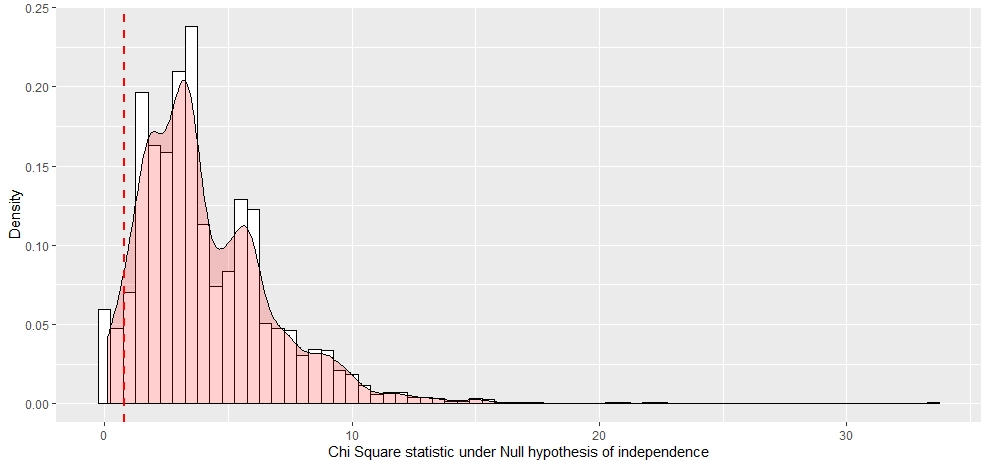
\includegraphics[width=\linewidth]{chisq.jpeg}
\end{center}


With same permutations, the p-value with Likelihood Ratio statistic turns to be exactly same, $0.9298$, which should be true, as both the statistic measure the same kind of deviations from independence setup.

\begin{lstlisting}[style = R-code]
	y <- perm.stat(meltdata, stat = "lrt", nperms = 5000, seed = 1911)
	head(y)
	paste("Approximated p-Value is", sum(y > lrt.stat(data))/5000)
\end{lstlisting}

\begin{lstlisting}[style = R-output]
	[1] 5.655498 6.280661 5.001904 2.184919 4.975902 3.566309
	[1] "Approximated p-Value is 0.9298"
\end{lstlisting}

and the null distribution looks as follows;

\begin{center}
	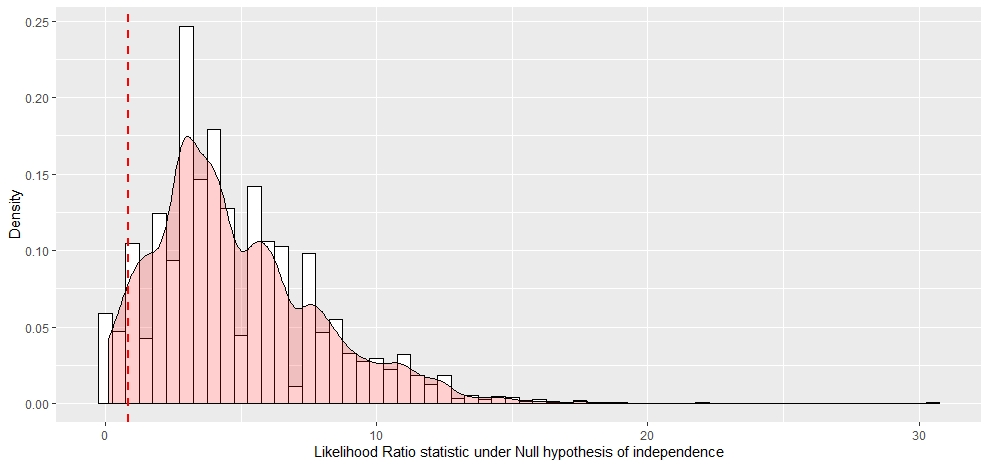
\includegraphics[width=\linewidth]{lrt.jpeg}
\end{center}

From the figures above, we find that the distribution of chi-square statistic is less dispersed than the null distribution of Likelihood ratio statistic. However, both the distributions are positively skewed, as expected and resembles the structure of a chi-square distribution.

Now, since both these p-values are $0.9298$ which is extremely higher than the significance level of $0.05$, hence we cannot reject the null hypothesis of independence between \textbf{Gender} and \textbf{Handedness}. As far as this data is concerned, it does not show any evidence that these two variables are associated in some way (i.e. not independent).

Also note that, the exact p-values obtained are extremely close to the approximate p-value based on asymptotic distribution of Pearson's chi-square and Likelihood Ratio test statistic. Clearly, it indicates that the asymptotic distribution well approximates the behavior of exact distribution in the light of the data.

Following is table containing the p-values for these permutation tests, based on the number of permutations used. All were produced with a seed of $1234$ in the previous functions.

\begin{center}
	\begin{tabular}{|c|c|c|}
		\hline
		Number of Permutations & p-value with Chi-Square statistic & p-value with LRT\\
		\hline
		5 & 1 & 1\\
		10 & 1 & 1\\
		50 & 0.92 & 0.92 \\
		100 & 0.93 & 0.93 \\
		500 & 0.932 & 0.932 \\
		1000 & 0.932 & 0.932 \\
		5000 & 0.9324 & 0.9324 \\
		10,000 & 0.9336 & 0.9336 \\
		100,000 & 0.93652 & 0.93652\\
		\hline 
	\end{tabular}	
\end{center}

Interestingly, the p-values for both type of test statistic for permutation test turns out to be same.

\end{solution*}
\vskip3pt
%%%%%%%%%%%%%%%%%%%%%%%%%%%%%%%%%%%%%%%%%%%%%%%%%%
% Problem 2
%%%%%%%%%%%%%%%%%%%%%%%%%%%%%%%%%%%%%%%%%%%%%%%%%%
\begin{problem}
\textbf{Exact logistic regression} \hfill [12]\vskip3pt\noindent
% Problem statement
In a standard binomial logistic regression set-up
\[
    \mathrm{logit}(\mathbb{P}(Y_i = 1)) = \beta_0 + \beta^\top X_i, \qquad  i = 1, \ldots, n, 
\]
write down sufficient statitsics $T_j$ for the parameters $\beta_j$, $j = 0, \ldots, p$. Show that the distribution of $T_p$ conditional on $T_0, \ldots, T_{p - 1}$ depends only on $\beta_p$. Thus, using this conditional distribution, one can estimate and perform inference on $\beta_p$. Does a conditional MLE always exist?

Write down the conditional distribution under $H_0: \beta_p = 0$. Describe how you would do an exact test of this hypothesis. 

Use the \textbf{R} packages \texttt{logistiX} and \texttt{elrm} to perform exact logistic regression on the data in Table~\ref{tab:admit} with ``White-collar job'' as response, and ``Gender'' and ``College education'' as explanatory variables.
\begin{table}[!htbp]
	\centering
	\begin{tabular}{cccc}
		Gender & College education & White-collar job & Number  of cases \\ \hline
		M & No & 1 & 8 \\
		F & No & 1 & 6 \\
		M & Yes & 7 & 10 \\
		F & Yes & 6 & 6
	\end{tabular}
	\caption{Another fictitious dataset.}
	\label{tab:admit}
\end{table}
Also, perform a standard logistic regression on the same data and compare the results.

\end{problem}
%%%%%%%%%%%%%%%%%%%%%%%%%%%%%%%%%%%%%%%%%%%%%%%%%%
% Solution to problem 2
%%%%%%%%%%%%%%%%%%%%%%%%%%%%%%%%%%%%%%%%%%%%%%%%%%
\begin{solution*}
% Write your solution here.

We write the likelihood of the binomial logistic regression setup, where $(X_i, Y_i)$ be the set of datapoints with $Y_i$ taking values $0$ and $1$. 

\begin{align*}
	\mathsf{L} & = \prod_{i=1}^{n} \left( \Pr(Y_i = 1) \right)^{Y_i} \left( \Pr(Y_i = 0) \right)^{1 - Y_i}\\
	& = \prod_{i=1}^{n} \left( \frac{e^{\beta_0 + \beta^\intercal X_i}}{1 + e^{\beta_0 + \beta^\intercal X_i}} \right)^{Y_i} \left( \frac{1}{1 + e^{\beta_0 + \beta^\intercal X_i}} \right)^{1 - Y_i}\\
	& = \prod_{i=1}^{n}\left(\frac{1}{1 + e^{\beta_0 + \beta^\intercal X_i}}\right) \times e^{\beta_0\sum_{i=1}^{n}Y_i + \sum_{j=1}^{p} \beta_j \sum_{i=1}^{n}X_{ij}Y_i}\\	
\end{align*}

where $X_{ij}$ is the $i$-th observation corresponding to $j$-th variable (or predictor). Note that, the first term in the multiplication does not depend on the random observation $Y_i$, and hence is a fixed function of the parameters $\beta$, (as $X_i$'s are treated as constants). Therefore, by use of Neymann Factorization theorem, we obtain that; $T = (T_0, T_1, \dots T_p)$ with $T_0 = \sum_{i=1}^{n}Y_i$ and $T_j = \sum_{i=1}^{n}X_{ij}Y_i$ is a sufficient statistic for $\left(\beta_0, \beta_1, \dots \beta_p\right)$. 

Note that, the joint density of $(T_0, T_1, \dots T_p)$ is; $f(t_0, t_1, \dots t_p) \propto \exp\left[ \sum_{j=0}^{p} \beta_jt_j\right]$. Therefore,

\begin{align*}
	f(t_p\vert  t_0, t_1, \dots t_{p-1}) & = \frac{f(t_0, t_1, \dots t_p)}{f(t_0, t_1, \dots t_{p-1})}\\
	& = \frac{f(t_0, t_1, \dots t_p)}{\sum_{t_p} f(t_0, t_1, \dots t_p)}\\
	& = \frac{c(t_0, \dots t_p)\exp\left[ \sum_{j=0}^{p} \beta_jt_j\right]}{\sum_{t_p} c(t_0, \dots t_p) \exp\left[ \sum_{j=0}^{p} \beta_jt_j\right]} \text{, where } c(t_0, \dots t_p) \text{ is the proportionality constant}\\
	& = \frac{c(t_{(p-1)}, t_p)\exp\left[\beta_pt_p\right]}{\sum_{t_p} c(t_{(p-1)}, t_p)\exp\left[\beta_pt_p\right]} \text{ where } t_{(p-1)} = (t_0, t_1, \dots t_{(p-1)})
\end{align*}

which does only depend on $\beta_p$. Also note that, the conditional MLE does not always exist. This can be seen as follows. Since $X_{ip}$'s are fixed quantities, and $Y_i$ is 0 or 1, it is clear that, the sum in the denominator runs through all elements of the set $\mathbb{T}_p = \left\{ \sum_{i=1}^{n}Y_iX_{ip} : Y_i \in \{0, 1\} \right\}$. Let, the observed $t^\ast_p$ that we get is $\max \mathbb{T}_p$, which exists since the set $\mathbb{T}_p$ is finite for a fixed set of $X_i$'s. Then;

\begin{align*}
	f(t^\ast_p \vert t_0, t_1, \dots t_{p-1}) & = \frac{c(t_{(p-1)}, t^\ast_p)\exp\left[\beta_pt^\ast_p\right]}{\sum_{t_p \in \mathbb{T}_p} c(t_{(p-1)}, t_p) \exp\left[\beta_pt_p\right]}\\
	& = \frac{1}{1 + \sum_{t_p \in \mathbb{T}_p - \{t^\ast_p\}} \frac{c(t_{(p-1)}, t^\ast_p)}{c(t_{(p-1)}, t_p)}\exp\left[\beta_p(t_p - t^\ast_p) \right]}\\
	& \rightarrow 1 \quad \text{as } \beta_p \rightarrow \infty \text{, since } (t_p - t^\ast_p) < 0
\end{align*}

Therefore, conditional MLE need not always exist in the above case. Also, note that the proportionality constants are positive. On the other hand, if the observed $t^{\ast\ast}_p$ that we obtain is actually $\min\mathbb{T}_p$, then;

\begin{align*}
f(t^{\ast\ast}_p \vert t_0, t_1, \dots t_{p-1}) & = \frac{c(t_{(p-1)}, t^{\ast\ast}_p)\exp\left[\beta_pt^{\ast\ast}_p\right]}{\sum_{t_p \in \mathbb{T}_p} c(t_{(p-1)}, t_p) \exp\left[\beta_pt_p\right]}\\
& = \frac{1}{1 + \sum_{t_p \in \mathbb{T}_p - \{t^{\ast\ast}_p\}} \frac{c(t_{(p-1)}, t^{\ast\ast}_p)}{c(t_{(p-1)}, t_p)}\exp\left[\beta_p(t_p - t^{\ast\ast}_p) \right]}\\
& \rightarrow 1 \quad \text{as } \beta_p \rightarrow -\infty \text{, since } (t_p - t^{\ast\ast}_p) > 0
\end{align*}

Hence, in this case also, the conditional MLE need not exist.

Under the null hypothesis $H_0 : \beta_p = 0$, the conditional distribution reduces to; $f_{H_0}(t_p \vert t_0, \dots t_{p-1}) = \frac{c(t_{(p-1)}, t_p)}{\sum_{u \in \mathbb{T}_p} c(t_{(p-1)}, u)}$. 

Now, to perform a hypothesis testing for $\beta = 0$, note that; $f_{T_p}(t; \beta_p)/f_{T_p}(t; \beta_p = 0) \propto \exp\left[ \beta_p t\right]$. As the likelihood ratio is monotonically increasing as a function of $t$, hence, we obtain the p-value for the observed value of the statistic $T_p = \sum_{i=1}^{n} Y_i X_{ip}$ as;

$$p_{+} = \sum_{u \geq t} f_{T_p}(u; \beta_p = 0) = \frac{\sum_{u \geq t} c(t_{(p-1)}, u)}{\sum_{u \in \mathbb{T}_p} c(t_{(p-1)}, u)}$$

for testing against the alternative $\beta > 0$. Similarly, for testing against the alternative that $\beta < 0$, we could obtain the p-value as; 

$$p_{-} = \sum_{u \leq t} f_{T_p}(u; \beta_p = 0) = \frac{\sum_{u \leq t} c(t_{(p-1)}, u)}{\sum_{u \in \mathbb{T}_p} c(t_{(p-1)}, u)}$$

And for testing against the two sided alternative; we can use the p-value as $2 \min\left\{  p_{+}, p_{-} \right\}$. Then, we use this p-values and compare them with the nominal significance level $\alpha$, to perform the hypothesis test (i.e. reject $H_0$ when the p-value is less than the significance level, and accept otherwise).

Next, we use package \texttt{elrm} to perform exact logistic regression on the given data.

\begin{lstlisting}[style = R-code]
	df <- data.frame(Gender = c("M","F","M","F"), CollegeEd = c("No", "No","Yes","Yes"), WhiteJob = c(1, 1, 7, 6), Total = c(8, 6, 10, 6))
	
	library(elrm)
	
	# CI for Gender variable
	fit <- elrm(WhiteJob / Total ~ Gender + CollegeEd, interest = ~ Gender, dataset = df, iter = 10e5, burnIn = 100)
	summary(fit)
	
	# CI for College Education Variable
	fit <- elrm(WhiteJob / Total ~ Gender + CollegeEd, interest = ~ CollegeEd, dataset = df, 
	iter = 10e5, burnIn = 100)
	summary(fit)
	
\end{lstlisting}

\begin{lstlisting}[style = R-output]
	Progress: 100%  Progress:  95%  Progress:  90%  Progress:  85%  Progress:  80%                  
	Generation of the Markov Chain required 35 secs
	Conducting inference ...
	Inference required 5 secs
	
	Call:
	
	elrm(formula = WhiteJob/Total ~ Gender + CollegeEd, interest = ~Gender, iter = 1e+06, dataset = df, burnIn = 100)
	
	
	Results:
	
			estimate 	p-value 	p-value_se 	mc_size
	GenderM -1.35482 	0.33699    	0.00094  	999900
	
	
	95% Confidence Intervals for Parameters
	
				lower    	upper
	GenderM 	-5.342778 	1.128712
	
	
	===================================================================
	Call:
	
	elrm(formula = WhiteJob/Total ~ Gender + CollegeEd, interest = ~CollegeEd, iter = 1e+06, dataset = df, burnIn = 100)
	
	
	Results:
	
					estimate 	p-value 	p-value_se 	mc_size
	CollegeEdYes   	3.6278 		0.00031     2e-05  		999900
	
	
	95% Confidence Intervals for Parameters
	
					lower    	upper
	CollegeEdYes 	1.107514 	7.948637
\end{lstlisting}

From the above confidence interval, we note that the for the Gender variable, the 95\% confidence interval does contain the value $0$, and hence we are unable to reject that null hypothesis. So, conclude that effect of Gender on probability of getting White Collar Job is insignificant based on the data. However, for the College Education variable, the 95\% exact confidence interval contains the value $0$, and hence we can reject the null hypothesis that coefficient for College Education in logistic regression model is $0$, and conclude that effect of College Education on probability of getting White Collar Job is significant at a 5\% level of significance.

Using the package \texttt{logistiX}, almost similar confidence intervals are obtained;

\begin{lstlisting}[style = R-code]
	library(logistiX)
	Gender <- factor(c(rep("M", 8), rep("F", 6), rep("M", 10), rep("F", 6)))
	CollegeEd <- factor(c(rep("No", 14), rep("Yes", 16)))
	WhiteJob <- c(1, rep(0, 7), 1, rep(0, 5), rep(1, 7), rep(0, 3), rep(1, 6))
	longdf <- data.frame(Gender = Gender, CollegeEd = CollegeEd, WhiteJob = WhiteJob)
	
	x <- model.matrix(WhiteJob ~ Gender + CollegeEd, longdf)[, -1]
	fit <- logistiX(x, y = longdf$WhiteJob)
	summary(fit)
\end{lstlisting}

\begin{lstlisting}[style = R-output]
	Exact logistic regression
	
	Call:
	logistiX(x = x, y = longdf$WhiteJob)
	
	Estimation method:           LX 
	CI method:                   exact  
	Test method:                 TST
	
	Summary of estimates, confidence intervals and parameter hypotheses tests:
	
	estimates     2.5 %   97.5 % statistic       pvalue cardinality
	1 -1.360474 -5.367983 1.128986         8 0.4556514914           6
	2  3.338699  1.101657 7.265954        13 0.0005817118          14
\end{lstlisting}

It seems that the \texttt{elrm} approximately obtains the same values of upper and lower bounds for confidence interval. Also, based on whether the confidence interval contains $0$ or not, or checking whether the p-value is less than $\alpha = 0.05$ or not, we obtain same decision as before. The contribution of \textbf{Gender} variable is not significant in deciding the probability of getting a \textbf{White Collar Job}, but the contribution of \textbf{College Education} is significant. 



We also perform the standard logistic regression on the data.

\begin{lstlisting}[style = R-code]
	fit <- glm(cbind(WhiteJob, Total - WhiteJob) ~ Gender + CollegeEd, data = df, family = "binomial")
	summary(fit)
\end{lstlisting}

\begin{lstlisting}[style = R-output]
	Call:
	glm(formula = cbind(WhiteJob, Total - WhiteJob) ~ Gender + CollegeEd, 
	family = "binomial", data = df)
	
	Deviance Residuals: 
	1        2        3        4  
	0.5628  -0.4437  -0.3179   0.9629  
	
	Coefficients:
					Estimate 	Std. Error 	z value 	Pr(>|z|)   
	(Intercept)   	-1.1471     0.8763  	-1.309  	0.19054   
	GenderM       	-1.4515     1.2038  	-1.206  	0.22790   
	CollegeEdYes   	3.6687     	1.1904   	3.082  		0.00206 **
	---
	Signif. codes:  0 '***' 0.001 '**' 0.01 '*' 0.05 '.' 0.1 ' '   1
		
	(Dispersion parameter for binomial family taken to be 1)
	
	Null deviance: 17.9365  on 3  degrees of freedom
	Residual deviance:  1.5418  on 1  degrees of freedom
	AIC: 13.877
	
	Number of Fisher Scoring iterations: 4
\end{lstlisting}

We note that, using Wald's asymptotic test for standard logistic regression, we also find that Gender does not have a significant effect, whereas College Education has one on predicting the log odds of having White Collar job.




\end{solution*}
\end{document}











